\documentclass{../../slides-style}

\slidetitle[CI]{Системы непрерывной интеграции}{}

\begin{document}
    
    \begin{frame}[plain]
        \titlepage
    \end{frame}

    \section{Введение}

    \begin{frame}
        \frametitle{Continuous Integration (1)}
        Непрерывная интеграция --- практика слияния всех изменений по нескольку раз в день, сборки их в известном окружении и запуска юнит-тестов.
        \begin{itemize}
            \item Автоматическая сборка
            \begin{itemize}
                \item Всё, что нужно для сборки, есть в репозитории, может быть получено на чистую (ну, практически) машину и собрано одной консольной командой
            \end{itemize}
            \item Большое количество юнит-тестов, запускаемых автоматически
            \item Выделенная машина, слушающая репозиторий и выполняющая сборку
            \begin{itemize}
                \item Чаще всего каждая сборка запускается на заранее настроенной виртуалке или контейнере
            \end{itemize}
        \end{itemize}
    \end{frame}

    \begin{frame}
        \frametitle{Continuous Integration (2)}
        \begin{itemize}
            \item Извещение всех разработчиков о статусе
            \begin{itemize}
                \item Если сборка не прошла, разработка приостанавливается до её починки
            \end{itemize}
            \item Автоматическое выкладывание
            \item Пока сборка не прошла, задача не считается сделанной
            \begin{itemize}
                \item Короткие билды (<10 мин.)
                \item deployment pipeline
                \begin{itemize}
                    \item Отдельная машина для сборки, для коротких тестов, для длинных тестов, для выкладывания
                \end{itemize}
            \end{itemize}
        \end{itemize}
    \end{frame}

    \begin{frame}
        \frametitle{Системы непрерывной интеграции}
        \begin{itemize}
            \item Локальные/on premises
            \begin{itemize}
                \item Jenkins --- очень старый, до сих пор активно используется, куча плагинов, стандарт де-факто в on premises CI
                \begin{itemize}
                    \item Некогда Hudson
                \end{itemize}
                \item JetBrains TeamCity --- тоже очень популярен
                \item GitLab CI --- если у вас и так GitLab, то почему нет
            \end{itemize}
            \item Облачные
            \begin{itemize}
                \item GitHub Actions
                \begin{itemize}
                    \item На самом деле, у всех нормальных облачных хостингов есть свои CI, даже у DockerHub
                    \item Azure Pipelines, Gitlab CI, Bitbucket Pipelines, ...
                \end{itemize}
                \item CircleCI
                \item AppVeyor --- очень удобен для Windows/Visual Studio
                \item Travis --- изначально для Linux
            \end{itemize}
        \end{itemize}
    \end{frame}

    \section{GitHub Actions}

    \begin{frame}
        \frametitle{GitHub Actions}
        \begin{itemize}
            \item Бесплатная система облачной сборки для проектов на GitHub
            \item \url{https://docs.github.com/en/actions}
            \item Как настроить:
            \begin{itemize}
                \item В репозитории на GitHub Settings -> Actions -> Allow all actions
                \item Создаём в корне репозитория папку .github/workflows/
                \item В нём создаём файл <имя действия>.yml (например, ci.yml)
                \item Описываем процесс сборки согласно \url{https://docs.github.com/en/actions/learn-github-actions/workflow-syntax-for-github-actions}
                \begin{itemize}
                    \item Пример и описание линуксовой сборки: \url{https://www.incredibuild.com/blog/using-github-actions-with-your-c-project}
                \end{itemize}
                \item Коммитим-пушим
                \item Смотрим статус коммита и пуллреквеста
            \end{itemize}
        \end{itemize}
    \end{frame}

    \begin{frame}
        \frametitle{Что получится}
        \begin{center}
            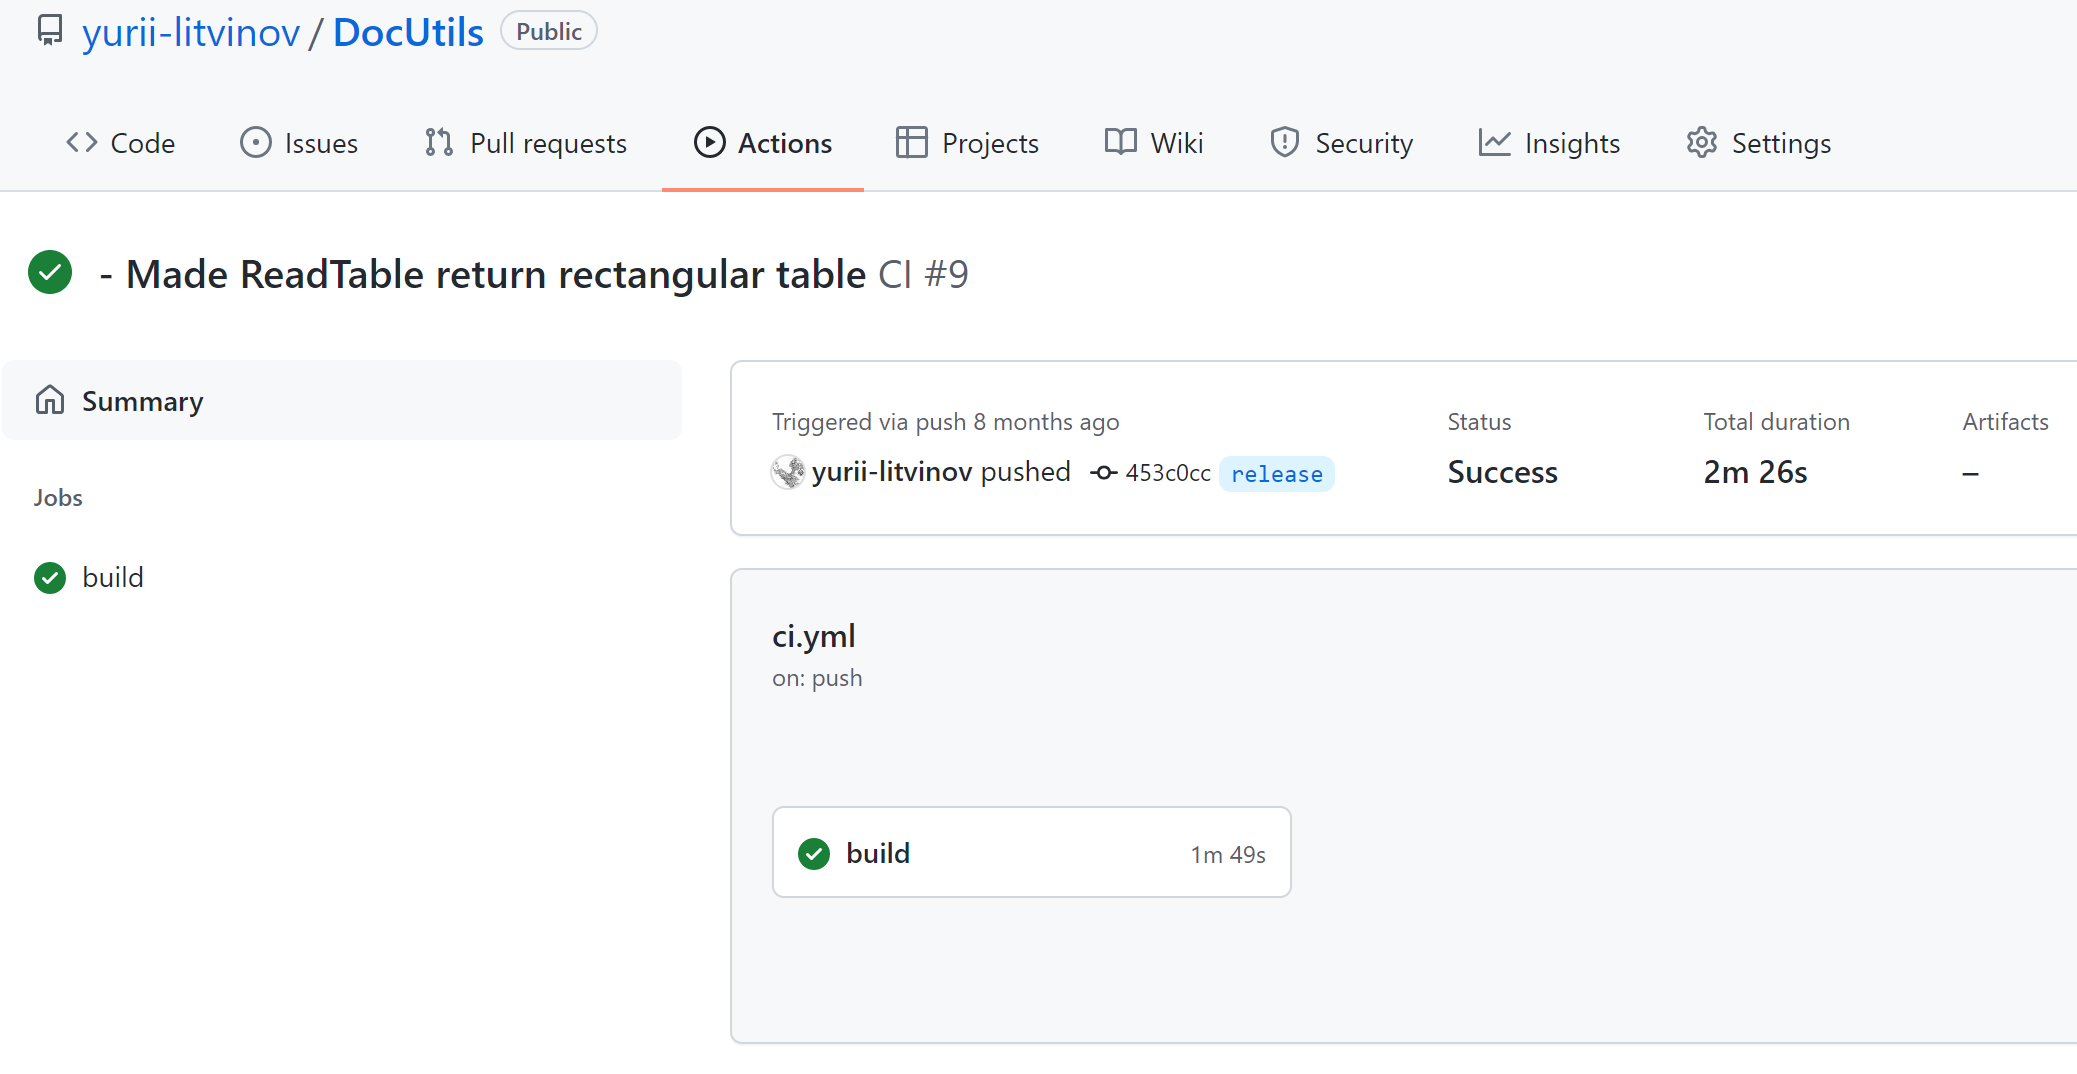
\includegraphics[width=0.9\textwidth]{githubActionsBuildStatus}
        \end{center}
        И появятся иконки статуса рядом с коммитами и пуллреквестами
    \end{frame}

    \begin{frame}[fragile]
        \frametitle{Типичный Workflow для сборки}
        \begin{scriptsize}
            \begin{minted}{yaml}
name: Build
on: [push, pull_request]
jobs:
    build-Ubuntu:
        runs-on: ubuntu-latest
        steps:
            - uses: actions/checkout@v2
            - uses: actions/setup-dotnet@v1
              with:
                  dotnet-version: '6.x'
            - name: Build
              run: for f in $(find . -name "*.sln"); do dotnet build $f; done
            - name: Run tests
              run: for f in $(find . -name "*.sln"); do dotnet test $f; done
    build-Windows:
        runs-on: windows-latest
        steps:
            ...
            - name: Build
              run: For /R %%I in (*.sln) do dotnet build %%I
            - name: Run tests
              run: For /R %%I in (*.sln) do dotnet test %%I
            \end{minted}
        \end{scriptsize}
    \end{frame}

    \begin{frame}
        \frametitle{GitHub Actions, Workflow и Job}
        \begin{center}
            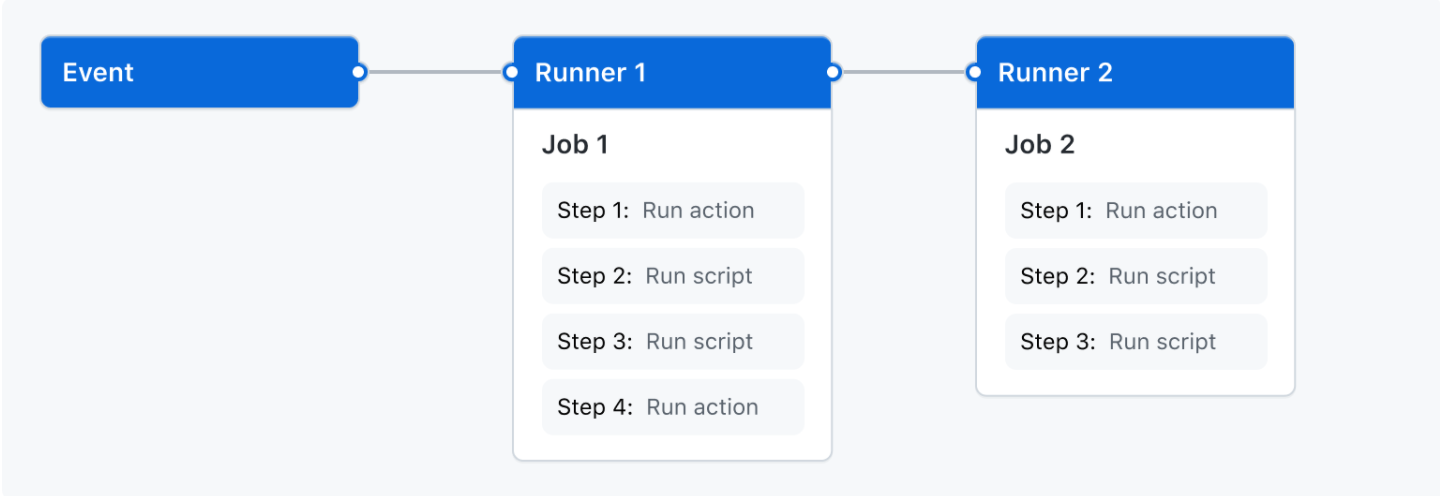
\includegraphics[width=0.7\textwidth]{githubActionsWorkflow}
        \end{center}
        \begin{itemize}
            \item Step --- это либо скрипт, либо \emph{Action}
            \item Action --- произвольный код (по сути, отдельное приложение), выполняющийся как шаг Job-а
            \begin{itemize}
                \item Переиспользуемый строительный блок
                \item Можно переиспользовать Workflow-ы
            \end{itemize}
        \end{itemize}
    \end{frame}

    \begin{frame}[fragile]
        \frametitle{Переменные окружения}
        \begin{scriptsize}
            \begin{minted}{yaml}
env:
  DAY_OF_WEEK: Monday

jobs:
  greeting_job:
    runs-on: ubuntu-latest
    env:
      Greeting: Hello
    steps:
      - name: "Say Hello Mona it's Monday"
        if: ${{ env.DAY_OF_WEEK == 'Monday' }}
        run: echo "$Greeting $First_Name. Today is $DAY_OF_WEEK!"
        env:
          First_Name: Mona
            \end{minted}
        \end{scriptsize}
    \end{frame}

    \begin{frame}[fragile]
        \frametitle{Матрица сборки}
        \begin{scriptsize}
            \begin{minted}{yaml}
runs-on: ${{ matrix.os }}
strategy:
  matrix:
    os: [ubuntu-18.04, ubuntu-20.04]
    node: [10, 12, 14]
steps:
  - uses: actions/setup-node@v2
    with:
      node-version: ${{ matrix.node }}
            \end{minted}
        \end{scriptsize}
    \end{frame}

    \begin{frame}
        \frametitle{Что ещё?}
        \begin{itemize}
            \item Секреты
            \begin{itemize}
                \item \mintinline{yaml}|super_secret: ${{ secrets.SUPERSECRET }}|
            \end{itemize}
            \item Кеширование промежуточных результатов
            \item Автоматическое развёртывание
            \begin{itemize}
                \item В том числе, автодеплой документации на github-pages
            \end{itemize}
            \item Проверка стиля кодирования, статический анализ кода и т.п.
            \begin{itemize}
                \item Может быть интересно для Python-разработчиков
            \end{itemize}
            \item Можно иметь несколько Workflow-ов в одном репозитории
        \end{itemize}
    \end{frame}

    \section{AppVeyor}

    \begin{frame}
        \frametitle{AppVeyor}
        \begin{itemize}
            \item \url{https://www.appveyor.com/} --- отдельная облачная CI-cистема, тоже довольно неплоха и проще в настройке
            \item Виртуальная машина с ОС Windows и настроенными инструментами сборки .NET-приложений
            \begin{itemize}
                \item Windows Server 2019 + VS 2022 или более старые
                \item Умеет Linux Ubuntu 20.04 и macOS 12.2.1
            \end{itemize}
            \item Интегрируется с GitHub-ом, Slack-ом, умеет деплоить
            \item Собирает по умолчанию системой сборки MSBuild
            \begin{itemize}
                \item Можно переубедить и собирать что угодно
            \end{itemize}
            \item Окружение настраивается конфигурационным файлом или <<вручную>> из скрипта сборки
        \end{itemize}
    \end{frame}

    \begin{frame}
        \frametitle{AppVeyor, настройка сборки}
        \begin{itemize}
            \item Зайти на \url{https://www.appveyor.com/} по GitHub-аккаунту
            \item Добавить проект (разрешив AppVeyor просматривать список репозиториев на гитхабе)
            \item Положить в корень репозитория файл appveyor.yml с конфигурацией сборки
            \begin{itemize}
                \item Пустой тоже ок, это конфигурация по умолчанию, ищет .sln в корне репозитория и пытается его собрать
            \end{itemize}
            \item Закоммитить и запушить, это инициирует процесс сборки
            \item Результаты будут видны прямо на GitHub, у каждого коммита и в пуллреквесте:
        \end{itemize}
        \begin{center}
            
\includegraphics[width=0.7\textwidth]{appVeyorSuccess.png}
        \end{center}
    \end{frame}

    \begin{frame}[fragile]
        \frametitle{AppVeyor, пример файла конфигурации}
        \begin{minted}{yaml}
image: Visual Studio 2022

before_build: 
    - nuget restore myCoolHomework/Homework.sln

build: 
    project: myCoolHomework/Homework.sln

test_script: 
    - dotnet test myCoolHomework/Homework.sln
        \end{minted}
    \end{frame}

    \section{Jenkins}

    \begin{frame}
        \frametitle{Jenkins}
        \begin{itemize}
            \item Работает локально
            \begin{itemize}
                \item Следовательно, требует настройки и хостинга
                \item Следовательно, может использоваться в корпоративном окружении
            \end{itemize}
            \item Имеет кучу плагинов на все случаи жизни
            \item Опенсорсный, очень популярен по сей день
            \begin{itemize}
                \item Начинался в 2005 в Sun как Hudson
            \end{itemize}
        \end{itemize}
    \end{frame}

    \begin{frame}[fragile]
        \frametitle{Jenkinsfile}
        \begin{minted}{groovy}
pipeline {
    agent any
    stages {
        stage('build') {
            steps {
                sh 'mvn --version'
            }
        }
    }
}
        \end{minted}
    \end{frame}

    \begin{frame}[fragile]
        \frametitle{Более продвинутые шаги}
        \begin{minted}{groovy}
pipeline {
    agent any
    stages {
        stage('Deploy') {
            steps {
                retry(3) {
                    sh './flakey-deploy.sh'
                }

                timeout(time: 3, unit: 'MINUTES') {
                    sh './health-check.sh'
                }
            }
        }
    }
}
        \end{minted}
    \end{frame}

    \begin{frame}[fragile]
        \frametitle{Jenkins и Docker}
        \begin{minted}{groovy}
pipeline {
    agent { docker 'maven:3.5.2-jdk-8-slim' }
    stages {
        stage('build') {
            steps {
                bat 'mvn --version'
            }
        }
    }
}
        \end{minted}
    \end{frame}

    \begin{frame}[fragile]
        \frametitle{Переменные окружения}
        \begin{footnotesize}
            \begin{minted}{groovy}
pipeline {
    agent any

    environment {
        DB_ENGINE    = 'sqlite'
        AWS_ACCESS_KEY_ID     = credentials('AWS_ACCESS_KEY_ID')
        AWS_SECRET_ACCESS_KEY = credentials('AWS_SECRET_ACCESS_KEY')
    }

    stages {
        stage('Build') {
            steps {
                sh 'printenv'
            }
        }
    }
}
            \end{minted}
        \end{footnotesize}
    \end{frame}

    \begin{frame}[fragile]
        \frametitle{Слежение за тестами}
        \begin{minted}{groovy}
pipeline {
    agent any
    stages {
        stage('Test') {
            steps {
                sh './gradlew check'
            }
        }
    }
    post {
        always {
            junit 'build/reports/**/*.xml'
        }
    }
}
        \end{minted}
    \end{frame}

    \begin{frame}[fragile]
        \frametitle{Деплой, ручное подтверждение}
        \begin{scriptsize}
            \begin{minted}{groovy}
pipeline {
    agent any
    stages {
        ...
        stage('Deploy - Staging') {
            steps {
                sh './deploy staging'
                sh './run-smoke-tests'
            }
        }
        stage('Sanity check') {
            steps {
                input "Does the staging environment look ok?"
            }
        }
        stage('Deploy - Production') {
            steps {
                sh './deploy production'
            }
        }
    }
}
            \end{minted}
        \end{scriptsize}
    \end{frame}

\end{document}